\scanpage{31}
\reversemarginpar
\margin{\figure{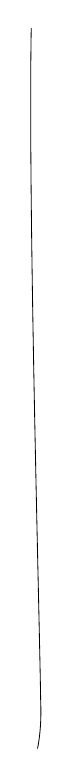
\begin{tikzpicture}[x=1cm,y=1cm]
\draw[line width=.3pt] (0,-.35) .. controls (-.04,-2.6) and (.10,-7.6) .. (.12,-8.9) .. controls (.13,-9.15) and (.11,-9.35) .. (.08,-9.5);
\end{tikzpicture}}}
\normalmarginpar
\uline{Théorème} 2.1.1. Soit $f:S'\handwritten{\longrightarrow}S$ un morphisme universellement localement \uline{$L$}-\unsure{1|l}-asphérique (SGA 4 XV \handwritten{1.11}), par exemple (SGA\handwritten{4}XV \handwritten{2.\unsure{1|2}}) un morphis\unsure{m} lisse, ou tel que $\deleted{\unsure{X}}\handwritten{S'}$ soit isomorphe à la limite\inserted{projective} d'un systême projectif\inserted{filtrant} de $S$-schémas lisses $S'_i$ à morphismes de transition affines\deleted{\unsure{,}} (SGA 4 XV \handwritten{1.13\inserted{(ii)}})

Soi\inserted{en}t $g:X\handwritten{\longrightarrow}S$ un morphisme de schémas, d'où un carré car\unsure{\deleted{ét}té|\deleted{té}ét}sien
% The four arrow shafts are handwritten; the objects and arrow labels are typed.
\diagram{\begin{tikzcd}[ampersand replacement=\&,column sep=large,row sep=large]
X \handwritten{\arrow[d,"g"']} \& X' \handwritten{\arrow[l,"f'"']} \handwritten{\arrow[d,"g'"]} \\
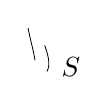
\begin{tikzpicture}[baseline=(s.base),x=1em,y=1ex]
\node[inner sep=0pt,anchor=base] (s) at (0,0) {$S$};
\draw[line width=.3pt] (-1.55,4.1) .. controls (-1.48,3.2) and (-1.35,2.2) .. (-1.30,1.4);
\draw[line width=.3pt] (-.95,2.65) .. controls (-.84,1.9) and (-.72,1.1) .. (-.87,.45);
\end{tikzpicture}
\& S'\handwritten{\arrow[l,"f"']}\rlap{,}
\end{tikzcd}}

$G$ un\inserted{ind-\uline{$L$}-} champ sur $X$\inserted{(\uline{V} \handwritten{5}\quad),} \deleted{dont les faisceaux d'automorphismes sont des ind-\uline{$L$}-faisceaux,} $G'=f'^{\handwritten{*}}(G)$ le champ image inverse sur $X'$.

\begin{enumerate}[label=\alph*)]
\item Si \deleted{$S$ et $S'$ sont strictement locaux et} $f$ est un morphisme \deleted{strictement} \uline{local} de schémas strictement locaux, alors le foncteur
\[
G(X)\handwritten{\longrightarrow}G'(X')
\]
est une équivalence de catégories.

\item Si $g$ est cohérent(i.e. quasi-compact et quasi-séparé) alors le morphisme de champs ``de changement de base''
\[
f^{\handwritten{'}}(g_{\handwritten{*}}(G))\handwritten{\longrightarrow}g'_{\handwritten{*}}(f'^{\handwritten{*}}(G))\deleted{\handwritten{\unsure{=g_*,|=g_*'}}}
\]
est une équivalence de champs sur $S'$.
\end{enumerate}

\reversemarginpar
\margin{\figure{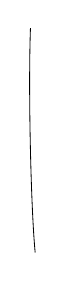
\begin{tikzpicture}[x=1cm,y=1cm]
\draw[line width=.3pt] (0,-.25) .. controls (-.03,-1.1) and (.01,-2.6) .. (.06,-3.1);
\end{tikzpicture}}}
\normalmarginpar
\uline{Corollaire} 2.1.2. Soient $k$ un corps séparablement clos, $k'$ une extension séparablement close de $k$, $X$ un $k$-schéma, $X'=X\handwritten{\otimes}_k k'$, alors pour tou\unsure{t} \deleted{champ $G$} ind-\uline{$L$}-champ $G$ sur $X$, désignant par $G'$ son image inverse sur $X'$, le foncteur
\[
G(X)\handwritten{\longrightarrow}G'(X')
\]
est une équivalence de catégories.

O\unsure{\deleted{p}n|\deleted{n}p} sait en effet (SGA 4 XVI\quad\quad) que $\operatorname{Spec}(k')\handwritten{\longrightarrow}\operatorname{Spec}(k)$ est universellement localement \uline{$L$}-1-asphérique.

Démonstration. On prouve a) par référence à SGA 4 XVI (nouvelle édition !)\inserted{\handwritten{et à $\overline{\text{\uline{V}}}$ - -}}, et b) en se ramenant à a) par des lemmes 2.1.7.2 et 2.1.7.4 renumérotés.
% Bottom marginal note, beginning beside the final proof line and continuing below it.
\par\noindent\hfill\begin{minipage}{.70\linewidth}
\handwritten{En tout, ça devrait faire 3 pages au Ch.p $\overline{\text{\uline{VII}}}$ au maximum, -- mais il y \unsure{aurait|aura} renvois au Ch.p $\overline{\text{\uline{V}}}$.}
\end{minipage}
% archive sheet number: 30
